\documentclass[tikz,border=3mm]{standalone}
\input{emerald_style.tex}
\begin{document}
\begin{tikzpicture}[x=1cm,y=1cm]
  \fill[ivory] (-.10,-.55) rectangle (16.10,7.65);
  \node[ctitle,text=nvdark] at (8,7.34) {Action-Conditioned Video World-Model Rollout};
  \node[csub,text=nvgraphite] at (8,6.94)
    {Teal marks observed context, emerald marks the generated horizon, and amber carries the action sequence and future mask.};

  % Photorealistic rollout dominates the composition.
  \node at (8,4.78) {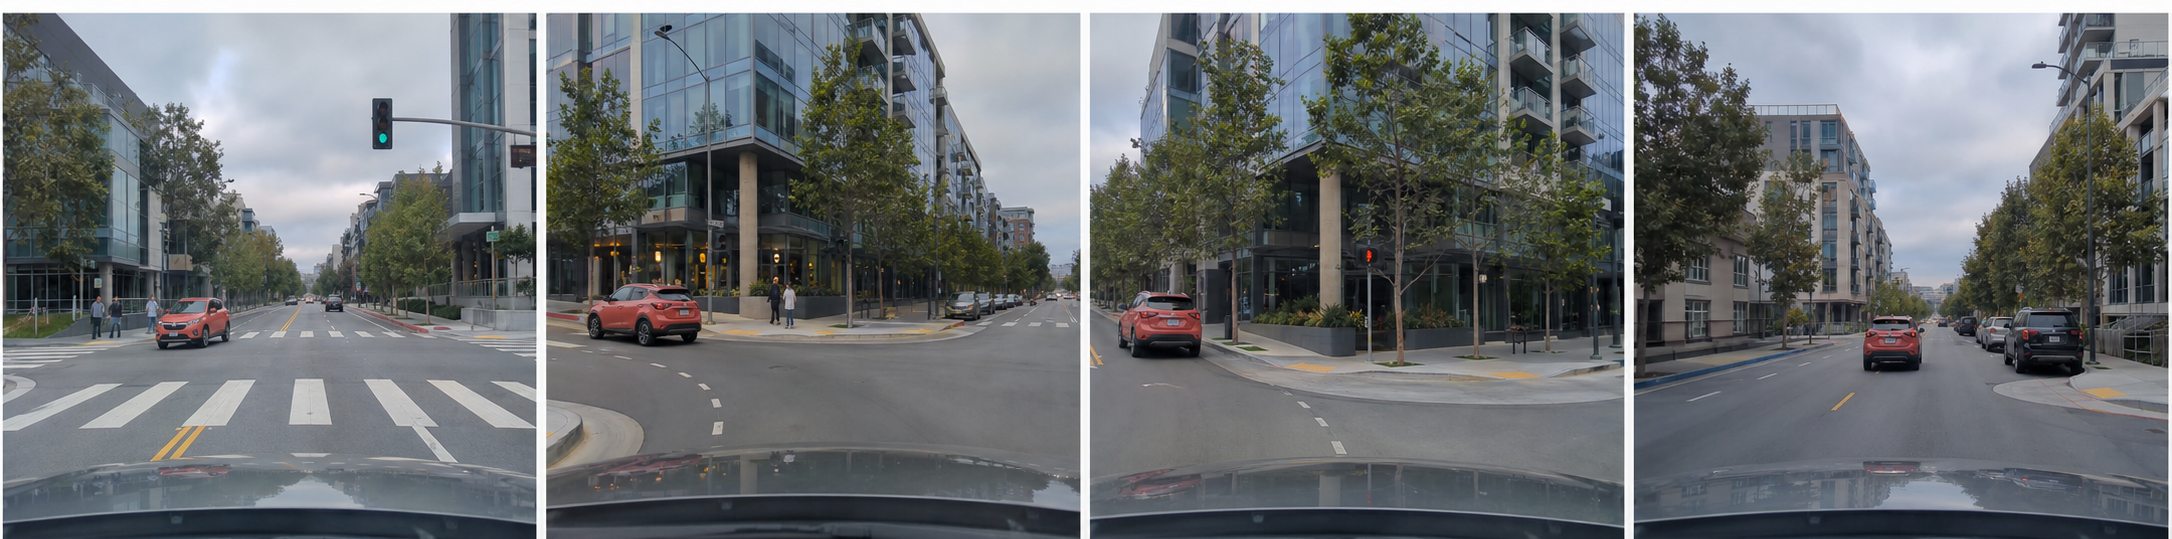
\includegraphics[width=14.85cm]{rollout_assets/urban_left_turn_rollout_crop.png}};
  \draw[draw=teal,line width=1.35pt] (.55,2.82) rectangle (4.22,6.74);
  \draw[draw=emerald,line width=1.35pt] (4.28,2.82) rectangle (15.45,6.74);
  \node[signal,signal from=west,signal to=east,fill=teal,draw=teal,
        text=white,ctiny,minimum width=1.75cm,minimum height=.43cm] at (1.52,6.44)
    {observed context};
  \node[signal,signal from=west,signal to=east,fill=emerald,draw=emerald,
        text=white,ctiny,minimum width=2.55cm,minimum height=.43cm] at (5.85,6.44)
    {generated future horizon};

  % Action tokens sit exactly on frame transitions.
  \foreach \x/\a/\txt in {4.25/$a_k$/{steer left},7.98/$a_{k+1}$/{continue left},11.71/$a_{k+2}$/{straighten}} {
    \node[circle,fill=amber,draw=nvdark,
          line width=.6pt,cmicro,minimum size=.58cm] at (\x,2.66) {\a};
    \node[cmicro,text=nvgraphite] at (\x,2.30) {\txt};
  }
  \node[cmicro,text=teal] at (2.38,2.26) {$c^{(k)}$};
  \node[cmicro,text=emerald] at (9.90,2.00)
    {$\hat y^{(k)}_{1:H}\sim p_\theta(\,\cdot\mid c^{(k)},a^{(k)}_{1:H})$};

  % Emerald-schematic context-forcing graph.
  \node[ctiny,text=nvgraphite,anchor=west] at (.45,1.65) {context-forcing distillation};
  \node[signal,signal from=west,signal to=east,fill=white,draw=teal,
        line width=1pt,ctiny,minimum width=2.65cm,minimum height=.70cm] (ctx) at (2.05,.94)
    {teacher-denoised context\\$\hat c_T=\tilde c-\eta v_T$};
  \node[rectangle,fill=white,draw=nvgraphite,line width=.7pt,ctiny,
        minimum width=2.15cm,minimum height=.66cm] (pack) at (5.10,.94)
    {pack $z=[\hat c_T;\tilde y]$\\$\tau=[0;t]$};
  \node[circle,fill=amber,draw=nvdark,line width=.65pt,cmicro,
        minimum size=.58cm] (action) at (5.10,1.68) {$a_{1:H}$};
  \draw[-Stealth,draw=amber,line width=.95pt] (action) -- (pack);

  \node[signal,signal from=west,signal to=east,fill=mint,draw=emerald,
        line width=1pt,ctiny,minimum width=2.20cm,minimum height=.58cm] (teach) at (7.70,1.30)
    {teacher target $\hat v_T$};
  \node[signal,signal from=west,signal to=east,fill=white,draw=teal,
        line width=1pt,ctiny,minimum width=2.20cm,minimum height=.58cm] (stud) at (7.70,.58)
    {student prediction $\hat v_S$};
  \node[diamond,aspect=1.35,fill=amber,draw=nvdark,line width=.65pt,
        ctiny,inner sep=2.0pt] (mask) at (9.72,.94) {$M$};
  \node[signal,signal from=west,signal to=east,fill=emerald,draw=emerald,
        text=white,ctiny,minimum width=2.65cm,minimum height=.76cm] (loss) at (11.95,.94)
    {future-only supervision};
  \node[circle,fill=amber,draw=nvdark,line width=.65pt,ctiny,
        minimum size=.88cm] (next) at (14.55,.94) {next\\chunk};

  \draw[-Stealth,draw=teal,line width=1pt] (ctx) -- (pack);
  \draw[-Stealth,draw=emerald,line width=1pt] (pack) -- (teach);
  \draw[-Stealth,draw=teal,line width=1pt] (pack) -- (stud);
  \draw[-Stealth,draw=emerald,line width=1pt] (teach) -- (mask);
  \draw[-Stealth,draw=teal,line width=1pt] (stud) -- (mask);
  \draw[-Stealth,draw=emerald,line width=1pt] (mask) -- (loss);
  \draw[-Stealth,draw=emerald,line width=1pt] (loss) -- (next);

  \draw[draw=emerald,line width=.75pt] (2.10,-.14) -- (13.95,-.14);
  \node[cmicro,text=nvgraphite,fill=ivory,inner xsep=7pt] at (8.05,-.14)
    {$\displaystyle M=[0_{\mathrm{context}};1_{\mathrm{future}}],
      \qquad
      \mathcal L_{\mathrm{CF}}
      =\frac{\sum_iM_i(\hat v_{S,i}-\hat v_{T,i})^2}
      {\max(1,\sum_iM_i)}$};
\end{tikzpicture}
\end{document}
